\documentclass[conference]{IEEEtran}
\IEEEoverridecommandlockouts
% The preceding line is only needed to identify funding in the first footnote. If that is unneeded, please comment it out.
\usepackage{cite}
\usepackage{amsmath,amssymb,amsfonts}
\usepackage{algorithmic}
\usepackage{graphicx}
\usepackage{textcomp}
\usepackage{xcolor}
\usepackage{hyperref}
\usepackage{pgfplots}
\usepackage{subfigure}
\usepackage{multirow}
\usepackage{booktabs}
\usepackage[utf8]{inputenc}
\usepackage{tikz} 
\usetikzlibrary{decorations.markings}

\pagestyle{plain}

\def\BibTeX{{\rm B\kern-.05em{\sc i\kern-.025em b}\kern-.08em
    T\kern-.1667em\lower.7ex\hbox{E}\kern-.125emX}}
    \pgfplotsset{compat=1.17}
    

\begin{document}

\title{Causal discovery for time series with latent confounders\\
\thanks{I thank Paul-Christian Buerkner for helpful discussions and
suggestions.}
}

\author{

\IEEEauthorblockN{Christian Reiser}
\IEEEauthorblockA{
\textit{University of Stuttgart}\\
Stuttgart, Germany \\
% st141151@stud.uni-stuttgart.de\\
christian.reiser@insightme.org
}

% \and

% \IEEEauthorblockN{Tanja Blascheck}
% \IEEEauthorblockA{
% \textit{University of Stuttgart}\\
% Stuttgart, Germany \\
% tanja.blascheck@vis.uni-stuttgart.de}

% \and

% \IEEEauthorblockN{Benedikt V. Ehinger}
% \IEEEauthorblockA{
% \textit{University of Stuttgart}\\
% Stuttgart, Germany \\
% benedikt.ehinger@vis.uni-stuttgart.de}

}

\maketitle

\begin{abstract}
Reconstructing the causal relationships behind the phenomena we observe is a fundamental challenge in all areas of science.
Discovering causal relationships through experiments is often infeasible, unethical, or expensive in complex systems. 
However, increases in computational power allow us to process the ever-growing amount of data that modern science generates.
This development has led to an emerging interest in the problem of causal discovery from observational data.
This work evaluates the LPCMCI algorithm, which aims to find generators compatible with a multi-dimensional, highly autocorrelated time series while some variables are unobserved.
Our numerical results find that LPCMCI performs best on auto-dependencies, then contemporaneous dependencies, and struggles most with lagged dependencies.
The source code of this project is available online\footnote{Sourcecode: \href{https://github.com/christianreiser/correlate/blob/master/causal_discovery/LPCMCI/compute_experiments.py}{https://github.com/christianreiser/correlate/blob/master/causal\_discovery/LPCMCI/compute\_experiments.py}}.
\end{abstract}

\begin{IEEEkeywords}
causal discovery, statistics
\end{IEEEkeywords}

%=============================================================================
\section{Introduction}
Reconstructing the causal relationships behind the phenomena we observe is a fundamental challenge in all areas of science. It helps to build physical models and predict the effect of interventions\cite{pearl_book_2018}.
The goal is to distinguish direct and indirect dependencies between variables, determine the dependencies' directionality, and identify common drivers.
The standard approach is to learn causal relationships through conducting experiments. However, interventions are often infeasible, unethical, or expensive in complex systems such as earth system science or healthcare\cite{runge_inferring_2019}.
Meanwhile, modern science generates a growing amount of data, which we can process due to increases in computational power.
The availability of data and abundance of computing power to process it has led to an emerging interest in the problem of causal discovery from observational data\cite{peters_elements_2018}.

In our work, we generate highly auto-correlated multi-dimensional time-series with latent variables that have similar properties to a dataset used in a study for mood prediction\cite{reiser_predicting_2022}. We briefly review methods that aim to reconstruct generators compatible with the observed data and elaborate on and evaluate a conditional independence constraint-based algorithm called LPCMCI\cite{gerhardus_high-recall_2021} in more detail.
%=============================================================================
\section{Problem description and notation}
\subsection{Preliminaries}
Consider a multivariate state generator that we want to reconstruct from data.
We assume it follows a vector-auto-regressive process\footnote{Auto-regressive process is a model, where the output variable depends only on its own lagged values and on a stochastic noise term. A \textit{vector-}auto-regressive process extends the auto-regressive model to multiple dimensions. As explained later, the output of our vector-auto-regressive process additionally depends on its current values.}, similar as used in \cite{gerhardus_high-recall_2021}, and described by the structural causal model (SCM)
\begin{equation}
V_{t}^{j}=f_{j}\left(pa\left(V_{t}^{j}\right), \eta_{t}^{j}\right) \quad \text { with } j=1, \ldots, \tilde{N},
\end{equation}
generating a multivariate time series $\mathbf{V}^{j}=\left(V_{t}^{j}, V_{t-1}^{j}, \ldots\right)$ for $j=1, \ldots, \tilde{N}$.
The functions $f_i$ describe mechanisms in the physical world which depend on a set of causal parents $p a\left(V_{t}^{j}\right) \subseteq\left(\mathbf{V}_{t}, \mathbf{V}_{t-1}, \ldots, \mathbf{V}_{t-p_{t s}}\right)$ and jointly independent noise variables $\eta_{t}^{j}$. $p_{t s}$ represents the maximal time lag between cause and effect.

We assume \textit{causal stationary}, which means that dependencies between all a pairs of variables $\left(V_{t-\tau}^{i}, V_{t^{}}^{j}\right)$ with the time lag $\tau \geq 0$ is the same as for all time shifted pairs $\left(V_{t^{\prime}-\tau}^{i}, V_{t^{\prime}}^{j}\right)$\cite{runge_causal_2018}. Therefore, causal stationarity simplifies the problem because it allows to reuse a momentary dependency found at one point in the time series and set its dependency to all other time shifted pairs.

We allow for \textit{contemporaneous} ($\tau=0$) effects because, in many applications, the measurement frequency is often slower than the time scale of the causal processes. Although there are contemporaneous effects, we still assume \textit{acyclicity}
, which means the causal graph has no cycles.
The SCM has \textit{latent variables}, which are variables in the data-generating SCM that are unobserved. We choose to include latent variables, because many real-world applications often only record a subset $\mathbf{X}=\left\{\mathbf{X}^{1}, \ldots, \mathbf{X}^{N}\right\} \subseteq \mathbf{V}=\left\{\mathbf{V}^{1}, \mathbf{V}^{2}, \ldots\right\}$ of the time series with $N \leq \tilde{N}$. 
However, we assume that no \textit{selection variables}, meaning there are no variables determining which measurements to include in or exclude from the data sample. Breaking this assumption can lead to selection bias and invalidate results.
Furthermore, we assume \textit{faithfulness}, meaning that conditional independence (CI) in the observed distribution $P(\bf{X})$ is due to the causal structure of the underlying process instead of mere chance\cite{gerhardus_high-recall_2021}.

\subsection{Implications of latent variables}
\label{sec:implLatent}
% latent DAGs -> infinite DAGs
This section explains the implications of latent variables, relying on graph theory.
While it briefly explains the graphical terminology, the interested reader can find more information about MAGs and PAGs in 

Data-generating processes are usually represented as graphs with directed edges that contain no directed cycles. Such graphs are called \textit{directed acyclic graphs (DAGs)}. Figure \ref{fig:DAGMAG}(a) shows a DAG with two latent variables, $H_1$ and $H_2$. Ideally we would like to reconstruct such DAGs from the data of its observed variables, here, $X_1$ and $X_2$. However, the reconstruction algorithms get no information about how many latent variables there are in the original DAG, and we do not restrict their number. Thus, the algorithm would search among an infinite number of DAGs.
\begin{figure}[htbp]
    \centering
    % true DAG
             \subfigure[Example of a DAG that represents a structural causal model with two hidden variables.]{
   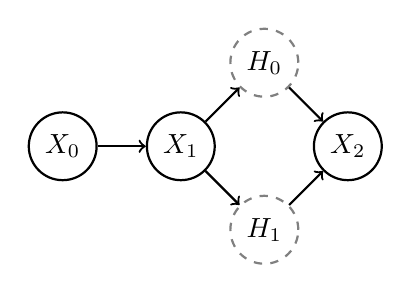
\begin{tikzpicture}[node distance={15mm}, thick, main/.style = {draw, circle}, hidden/.style = {draw=gray,dashed, circle}] 
\node[main] (0) {$X_0$}; 
\node[main] (1) [right of=0]{$X_1$}; 
\node[hidden] (2) [above right of=1] {$H_0$}; 
\node[hidden] (3) [below right of=1] {$H_1$}; 
\node[main] (4) [above right of=3] {$X_2$}; 
\draw[->] (0) -- (1); 
\draw[->] (1) -- (2); 
\draw[->] (1) -- (3); 
\draw [->](2) -- (4); 
\draw [->](3) -- (4); 
\end{tikzpicture}}\hspace{5mm}
% MAG
    \subfigure[The MAG over the observed variables of the DAG.]{
   \begin{tikzpicture}[node distance={15mm}, thick, main/.style = {draw, circle}, hidden/.style = {draw=gray,dashed, circle}] 
\node[main] (0) {$X_0$}; 
\node[main] (1) [right of=0]{$X_1$}; 
\node[main] (4) [above right of=3] {$X_2$}; 
    \draw[->] (0) -- (1); 
    \draw[<->] (1) -- (4); 
\end{tikzpicture}}\hspace{5mm}
% PAG
    \subfigure[Oracle PAG]{
   \begin{tikzpicture}[node distance={15mm}, thick, main/.style = {draw, circle}, hidden/.style = {draw=gray,dashed, circle}, o/.style={
        shorten >=#1,
        decoration={
            markings,
            mark={
                at position 1
                with {
                    \draw circle [xshift=-#1,radius=#1];
                }
            }
        },
        postaction=decorate
    },
    o/.default=2pt] 
\node[main] (0) {$X_0$}; 
\node[main] (1) [right of=0]{$X_1$}; 
\node[main] (4) [above right of=3] {$X_2$}; 
    \draw[->] (0) -- (1); 
    \draw[o] (1) -- (0); 
    \draw[o] (1) -- (4); 
    \draw[<-] (1) -- (4); 
\end{tikzpicture}
    }
    \caption{Two types of graphs that represent a structual causal models with latent variables.}
        \label{fig:DAGMAG}
\end{figure}
% ###
% MAG
% ###
Instead, as in the example of Figure \ref{fig:DAGMAG}(b), one can represent each DAG with latent variables compatible with the observed data by a \textit{maximal ancestral graph (MAG)} over the observed variables, which illustrates variables that are conditionally dependent due to latent confounding with bi-directed edges ($\leftrightarrow$)\cite{richardson_ancestral_2002}. 
% semantics ->  <->
MAGs are similar to DAGs but have the following differences in semantics. In a MAG, the tail (-) of an arrow, as in A $\rightarrow$ B, says that A is an ancestor of B. An arrowhead ($<,>$), like the one pointing on B, specifies that B is not an ancestor of A. Also, it does not exclude the possibility that A and B might be related due to latent confounding.
Since an arrowhead in a MAG declares the variable next to it as a non-ancestor, bidirectional edges ($\leftrightarrow$) exclude both variables from being the ancestor of the other variable and thus propose latent confounding between the two.

% Markov equivalence
\begin{table}[htbp] 
\begin{center}
    \caption{Chains of both directions and a forks cannot be differentiated via conditional independence. However, they can be differentiated from colliders. $X\!\perp\!\!\!\perp Y$ and $X\!\perp\!\!\!\perp Y|Z$ denote independence and conditional independence between the random variables X and Y, respectively.}
\begin{tabular}{@{}l|lll|l@{}}
\toprule
Name         & Chain   & Chain   & Fork    & Collider \\ \midrule
    Graph & $X\rightarrow Z \rightarrow Y$ & $X\leftarrow Z \leftarrow Y$ & $X\leftarrow Z \rightarrow Y$ & $X\rightarrow Z \leftarrow Y$ \\
    Independence & $X\not\!\perp\!\!\!\perp Y$    & $X\not\!\perp\!\!\!\perp Y$    & $X\not\!\perp\!\!\!\perp Y$   & $ \bf{X\!\perp\!\!\!\perp Y}  $       \\
    CI           & $X\!\perp\!\!\!\perp Y|Z$   & $X\!\perp\!\!\!\perp Y|Z$   & $X\!\perp\!\!\!\perp Y|Z$  & $\bf{X\not\!\perp\!\!\!\perp Y|Z}$      \\
    Equivalence & \multicolumn{3}{l|}{Markov equivalence class} & other Markov equivalence class \\ \bottomrule
\end{tabular}
        \label{tab:equiq}
\end{center}
\end{table}
CI-based methods cannot differentiate all MAGs \cite{richardson_ancestral_2002}. Graphs that contain the same CI information, are summarized in a class called \textit{Markov equivalent class}. Table \ref{tab:equiq} shows examples of Markov equivalence for cases without latent confounding. The interested reader can find a full explanation in section 3.6 about the equivalence of m-separation in Richardson and Spirtes, 2002 \cite{richardson_ancestral_2002}, which includes latent confounding. 
Since it is often not possible to find the MAG over the observed variables with CI-based methods, we aim to find all MAGs that satisfy the CI information. All these possible MAGs can be summarized in one graph, represented by a \textit{partial ancestral graph (PAG)}\cite{zhang_causal_2008}.
As Figure \ref{fig:DAGMAG}(c) shows, a PAG can represent uncertainty weather a link has an arrowhead ($<$ or $>$) or tail (-) with a circle-head ($\circ$). For example, the link C $\circ$$\rightarrow$ D says that D is not an ancestor of C, but we do not know if C is an ancestor of D or not. 
This case leaves us with three possibilities. First, there could be a directed path from C to D, second, the dependency could only be due to latent confounding, or third, it could be a combination of both. 

It is difficult to find the PAG that satisfies all conditional independencies because CI tests can fail due to limited sample size and low signal-to-noise ratios.
Nevertheless we evaluate the performance of the algorithm against this PAG that satisfies all CI information over the observed variables perfectly. We call this perfect PAG \textit{oracle PAG}, and it serves as our ground truth.
Figure \ref{fig:DAGMAG}(c) shows the oracle PAG of the previous example. 

To summarize, the goal is to find the PAG, which represents all MAGs that satisfy the conditional independence information over the observed variables.
% because we cannot identify the one original DAG due to Markov equivalence and latent confounders.


\section{Introduction into methods}

Granger causality can infer the causal structure of time series. Intuitively we say that X Granger-causes Y when the prediction of Y from its past is improved by accounting for X's past.
Then Y has to be dependent on the past of X given its own past. Formally that is
\begin{equation}
X \text { Granger-causes } Y: \Longleftrightarrow Y_{t} \not\!\perp\!\!\!\perp X_{\operatorname{past}(t)}  \mid Y_{\operatorname{past}(t)},
\end{equation}\cite{peters_elements_2018} where $\not\!\perp\!\!\!\perp$ denotes dependence and $|$ means 'conditioned on'.
Clive Granger himself extended Granger causality to a multivariate setting\cite{granger_testing_1980}. However, it can be misleading with the presence of instantaneous effects \cite{granger_clive_recent_1988} and requires that all variables are observed\cite{granger_testing_1980}.

FullCI determines the absence of a link between one variable $X_{t-\tau}^{i}$ with time lag $\tau$ and another variable $X_{t}^{j}$ by testing for their independence while conditioning on the past of all other variables $\mathbf{X}_{t}^{-} \backslash\left\{X_{t-\tau}^{i}\right\}$. 
Formally that is
$X_{t-\tau}^{i} $
$\!\perp\!\!\!\perp X_{t}^{j} $
$\mid \mathbf{X}_{t}^{-}$
$ \backslash\left\{X_{t-\tau}^{i}\right\}$ \cite{runge_pcmci_2019}.
A problem is that high dimensionality of the conditioning set decreases the detection power of FullCI \cite{runge_pcmci_2019}.
Usually the researcher decreases dimensionality by restricting the maximal time-lag $\tau_{max}$ through background knowledge or sets it to the largest time-lag with significant unconditional dependence\cite{runge_pcmci_2019}.
It is actually sufficient to condition only on the parents of the two variables\cite{pearl_causality_2000}, which allows decreasing the dimensionality of the conditioning set further, especially if the true graph is sparse.

The PC algorithm, named after its inventors Peter and Clark, is well known to exploit sparsity by iteratively using small conditioning sets\cite{runge_pcmci_2019}. However, when the size of the conditioning set is very limited, chances increase that true parents are not in the conditioning sets and false-positive links tend to remain\cite{runge_pcmci_2019}.

The PCMCI algorithm first runs a version of the PC algorithm adapted for time series, which removes most false links very efficiently, with the trade-off that some false positives remain\cite{runge_pcmci_2019}. In the second step, it tests for momentary conditional independence (MCI)
\begin{equation}
\mathrm{MCI}: X_{t-\tau}^{i} \not\!\perp\!\!\!\perp X_{t}^{j} \mid \left[[{pa}\left(X_{t}^{j}\right) \backslash\left\{X_{t-\tau}^{i}\right\}], {pa}\left(X_{t-\tau}^{i}\right)\right]
\end{equation}
to remove the remaining false links\cite{runge_pcmci_2019}.
This results in faster runtime and increased detection power than FullCI\cite{runge_pcmci_2019}.
PCMCI allows for multivariate and highly auto-dependent time-series. It's extension PCMCI+ also handles contemporaneous links. However, PCMCI and PCMCI+ are both assume the absence of latent confounders.

An algorithm that allows for latent confounders is the Fast Causal Inference algorithm (FCI)\cite{spirtes_causation_2000}. It is constraint-based and outputs a PAG which represents possible MAGs.
The tsFCI algorithm adapts FCI to time-series \cite{entner_causal_2010}. It extends FCI by additionally exploiting that causes precede effects. Furthermore, it assumes stationarity which allows applying a found momentary dependency between a pair of variables to be the same for all other shifted pairs.

So war we discussed methods that restrict the set of possible graphs via conditional independence and time ordering. As mentioned in section \ref{sec:implLatent}, the major downside of conditional independence-based methods is that they cannot differentiate Markov equivalent graphs. 
But it is possible to differentiate Markov equivalent models if they are Linear Non-Gaussian Acyclic Models (LiNGAMs).
In the bi-variate case, if the true SCM is 
\begin{equation}
Y=\alpha X+N_{Y}, \quad N_{Y} \!\perp\!\!\!\perp X
\end{equation}
with continuous random variables $X, Y$, and $N_Y$, then there exist no $\beta\in\mathbb{R}$ and random variable $N_X$ for the SCM in the reverse direction
\begin{equation}
X=\beta Y+N_{X}, \quad N_{X} \!\perp\!\!\!\perp Y
\end{equation}\cite{peters_elements_2018}.
The reason is that the LiNGAMs of both causal directions would be two dependent linear combinations of independent non-gaussian distributed random variables with non-zero coefficients. But the contrapositive of the Darmois–Skitovich theorem\cite{skitovich_linear_1954} says that such a linear combinations cannot exist.
Bi-variate LiNGAMs algorithms test in which direction the requirement of independent noise is broken $(\quad N_{Y} \!\perp\!\!\!\perp X$ or $\quad N_{X} \!\perp\!\!\!\perp Y)$, by regressing the data in both directions linearly. Residuals of the causal direction are independent and the residuals in the anti-causal direction depend on the input variable. 
The interested reader can find further details and visualizations in \cite{neal_introduction_2020} p. 108, a mathematical proof for the bi-variate case in the Appendix C.1 of \cite{peters_elements_2018}, and a proof for the multivariate case in \cite{shimizu_linear_2006}.

TS-LiNGAM is an algorithm based on LiNGAM but adapted for time series\cite{hyvarinen_causal_2008}. Like LiNGAM, it assumes linear dependencies and non-Gaussian noise. Since it can identify structure within the Markov equivalence class without relying only on time-ordering, it may have an advantage in handling contemporaneous links.
Limitations of TS-LiNGAM are the restriction to linear relationships, non-Gaussian noise, and instantaneous effects\cite{peters_causal_2013}. Furthermore, Peters et al. shows that TS-LiNGAM may fail when there is latent confounding. In their example of $X\leftarrow Z \rightarrow Y$ with the latent variable $Z$, they show how LiNGAM wrongly infers $X\rightarrow Y$\cite{peters_causal_2013}.

\section{Detection power and LPCMCI}
The main challenge of constraint based methods is increasing detection power, which quantifies the probability of finding a true link between two nodes.
The detection power of conditional independence based methods can be increased by
\begin{itemize}
    \item increasing the number of samples in the dataset \cite{gerhardus_high-recall_2021}, which results in more reliable CI tests,
    \item decreasing the dimensionality of the problem\cite{runge_pcmci_2019},
    \item increasing the causal effect size between the two variables\cite{gerhardus_high-recall_2021},
    \item increasing the statistical significance level of the conditional independence test\cite{gerhardus_high-recall_2021}, and
    \item decreasing the size of the conditioning set until it consists only of the parents of the two variables\cite{runge_pcmci_2019}.
\end{itemize}

In real-world applications, it is often possible to take more samples, decrease the problem's dimensionality by excluding irrelevant variables through expert knowledge, and increase the effect size by enhancing the signal-to-noise ratio of the measurements.
However, these properties are of less interest when developing methods and are usually fixed through the dataset.

Typically, the researcher allows a certain false positive rate that determines the significance level \cite{gerhardus_high-recall_2021}.
However, one can relax the statistical significance level of the conditional independence tests, which usually increases detection power.
Nevertheless, the downside is that it increases the risk of detecting more false links.
Furthermore, these false links in later steps can also decrease detection power. The reason is that later CI tests of true links might condition on these false links and reduce the CI scores of the true links. Each score that falls below the significance level $\alpha$ leads to the false removal of a true link. More intuitively, false links can "explain away" the effect of true links and thus remove them.
In our test case, we are less interested in keeping the false positive rate strictly below a specific value at the cost of much higher false negative rates. We rather optimize alpha to minimize true positives and true negatives equally strong. More details follow in chapter \ref{sec:eval}.

The LPCMCI (for Latent PCMCI) algorithm improves its performance by decreasing the size of the conditioning sets by discarding conditioning sets containing known non-ancestors of the two variables but including their known parents\cite{gerhardus_high-recall_2021}. It is challenging to do so because the conditioning sets have to contain the parents of the two variables before the CI-tests are completed. This order is not the case for predecessor algorithms. They first conduct the CI test and then orient the links. Only the latter yields parenthoods.
To overcome the challenge that ancestries and parentships are unknown, LPCMCI entangles CI tests with edge orientation to identify parentships. Each time the algorithm gains new knowledge about parent- or ancestorship, it updates its conditioning sets. After the algorithm converges once, it re-initializes the graph but keeps the identified parentships. 
It applies the same process again but extends the conditioning sets with the previously identified parents.
This procedure should remove most spurious links during the second run and assign edgemarks to the remaining links. 
However, the resulting graph tends to contain false links between variables that are dependent due to latent confounding. 
To remove them, the algorithm applies one more round of CI test and edge orientations with a modified rule to select conditioning sets\footnote{For more information on these modified conditioning sets, read about the $napds_t$ sets in definition S5 of\cite{gerhardus_high-recall_2021}.} 
to identify latently confounded links\cite{gerhardus_high-recall_2021}.

% when no autocorrelation: sufficient to condition on parents (Markov property)
% With autocorrelation: often given only one repetition of the time series with finitely many time points — this differs from the usual i.i.d. setting, in which we observe every variable several times. 
%With autocorrelation, the unknown true distribution has fewer degrees of freedom and will be typically wider than the assumed null distribution, leading to more false positives. -> also condition on lagged parents (parent of a parent) to account for autocorrelation
%=============================================================================

\section{Experiments}
The motivation of our work is to discover the causal dependencies in a real-world dataset about a persons mood and measurements from several consumer services and devices (e.g. sleep, nutrition, weather)\cite{reiser_predicting_2022} with the PCMCI algorithm. 
However, it is difficult to evaluate against this real-world dataset as the ground truth of its causal dependencies is unknown. Therefore, we apply the LPCMCI algorithm on simulated datasets with similar properties and known ground truth.

\subsection{Data-generation}
The synthetic data generating SCMs are given by
\begin{equation}
V_{t}^{j}=a_{j} V_{t-1}^{j}+\sum_{i} c_{i} f_{i}\left(V_{t-\tau_{i}}^{i}\right)+\eta_{t}^{j} \quad \text { for } \quad t \in\{1, \ldots, T\}, \quad j \in\{1, \ldots, \tilde{N} \}.
\end{equation}
The model consists of $\tilde{N}=11$ variables $V_t^j$. Three of these variables are selected at random and become latent later on.
Every variable $V_t^j$ has a linear auto-dependency $a_j V_{t-1}^{j}$, with $a_j \sim \mathcal{U}(0.3,0.6)$, meaning that the strength of the auto-dependency is drawn from a uniform distribution with a lower bound of 0.3 and an upper bound of 0.6.
In total there are $11$ randomly chosen variable pairs $(V_t^j,V^i_{t-\tau_i})$ with non-zero linear cross-dependencies $f_i \sim \pm \mathcal{U}(0.2,0.5)$. Otherwise $f_i=0$, meaning that all other variables have no cross-dependency.
60\% of links are instantaneous, meaning they have a time-lag of $\tau =0$. The other 40\% have a time-lag of $\tau=1$.
% The noises are drawn from a normal distribution with zero mean and variance drawn uniformly between 0.5 and two. Formally that is 
The noises $\eta^{j} \sim \mathcal{N}(0,\mathcal{U}[0.5,2])$.
Every SCM generates a discrete time-series of length T = 500. The experiment uses data of 4000 SCM. If a SCM generates a non-stationary time-series it is redrawn. This can happen when there is a positive feedback loop in the SCM that leads to a non-stationary trend in the data.

\subsection{Evaluation metrics}
\label{sec:eval}
Recall from section \ref{sec:implLatent} that we do not try to reconstruct the DAG that represents the original data-generating SCM. Instead we aim to find and evaluate against the oracle PAG, which is the PAG that satisfies all conditional independence information of the observed variables. 
The evaluation metrics distinguish between auto-dependencies and cross-dependencies. 
Furthermore, cross-dependencies are separated into contemporaneous links and lagged links, whereas auto-dependencies always have a lag, as contemporaneous auto-dependencies would violate the assumption of acyclicity.
% Note that the dimensionality of adjacencies is $(tau\_max*2 * N) + N$, because for every variable there can be an adjacency to every other variable can be an adjacency for each $tau$ in both directions plus one contemporaneous dimension with can 
Furthermore, we distinguish dependencies on whether adjacencies and their correct edgemarks are detected or not. In contrast to the oracle PAG, the LPCMCI can additionally return conflict edgemarks ("x"), although they will always be evaluated as false positives.
A conflict during edge orientation occurs when orientation rules of two variable triples propose to orient a common edgemark as both tail and head\cite{runge_pcmci_2020}. The underlying problem would be insufficient sample size or at least one assumption violation\cite{runge_tigramite_2022}.

We measure \textit{recall} and \textit{precision} of the adjacency and edge-orientation predictions. Recall (also known as \textit{sensitivity} measures the rate that a true link or adjacency is detected. Precision (also known as \textit{specificity} measures the rate that a predicted link is actually there.) Formally, that is $recall = \frac{tp}{tp+fn}$ and $precision = \frac{tp}{tp+fp}$, where
$tp$ stands for true positives, which is the number of edgemarks and adjacencies that are in the oracle PAG as well as the predicted PAG.
$fn$ stands for false negatives,  the number of adjacencies or edgemarks in the oracle PAG but not in the predicted PAG.
$fp$ stands for false positives, the number of adjacencies or edgemarks in the predicted PAG but not in the oracle PAG.
By this definition, each adjacency-$fn$ leads to two missing edgemarks, which increases the edgemark-$fn$ by two.
Also, vice versa, each adjacency-$fp$ leads to an increase of edgemark-$fp$ by two.

In order reduce the problem to a single-objective optimization problem, we aggregate the objectives of precision and recall of edgemarks and adjacencies to a single score via the harmonic mean:
\begin{equation}
harmonic\_score=\frac{4}{\frac{1}{recall\_adjacencies}+\frac{1}{precision\_adjacencies}+\frac{1}{recall\_edgemarks}+\frac{1}{precision\_edgemarks}}.
\label{eq:harmonicscore}
\end{equation}
We also used this $harmonic\_score$ as the objective to optimize the significance level $\alpha=0.26$. More specifically, we decreased the number of SCM realizations from 4000 to 50 to increase speed and searched manually for an $\alpha$ that leads to the best $harmonic\_score$.

Note that if the algorithm predicts the original data-generating DAG, the evaluation would still return a non-perfect score if the predicted DAG differs from the oracle PAG, even though the oracle PAG includes the predicted DAG. More specifically, the observed variables over the original DAG of the data-generating SCM is always included in the oracle PAG. But the oracle PAG is often larger, as it includes all MAGs that satisfy the CI information over the observed variables, even if their adjacencies are not in the data-generating DAG. Since the oracle PAG serves as ground truth, every adjacency that is not predicted but in the oracle PAG is evaluated as a false negative, even when it is not in the data-generating DAG.
For example, Figure \ref{fig:predicted}(b) shows an adjacency from node 6 to 8 which is not in the data-generating DAG of \ref{fig:predicted}(a). Figure \ref{fig:predicted}(c) shows that this adjacency is not detected, thus, the missing adjacency is evaluated as a false negative.


\subsection{Numerical Results}
\begin{table}[!htb]
    \caption{Numerical results}
    \begin{minipage}{.5\linewidth}
        \caption[]{precision and recall of edgemarks and adjacencies, which are further distinguished between lagged, auto-dependent, and contemporaneous links.}
      \centering
        \begin{tabular}{@{}llll@{}}
            \toprule
            \textbf{}                  &         & precision      & recall  \\ \midrule
            \multirow{4}{*}{adjacency} & auto    & 1.00             & 1.00       \\
                                       & contemp & 0.60             & 0.77       \\
                                       & lagged  & 0.38             & 0.39       \\
                                       & total   & 0.62             & 0.67       \\ \midrule
            \multirow{4}{*}{edgemark}  & auto    & 0.74             & 0.73       \\
                                       & contemp & 0.34             & 0.44       \\
                                       & lagged  & 0.27             & 0.26        \\
                                       & total   & 0.42             & 0.46       \\ \bottomrule
            \end{tabular}
            \label{tab:precision_recall}
    \end{minipage}%
    \begin{minipage}{.5\linewidth}
      \centering
            \caption[]{Rate of conflicting and unoriented edgemarks, which are further distinguished between lagged, auto-dependent, and contemporaneous links.}
            \begin{tabular}{@{}llll@{}}
            \toprule
            \textbf{}                        &         & conflict rate    & unorianted rate  \\ \midrule
            \multirow{4}{*}{conflict rate}   & lagged  & 0.00               & 0.14                \\
                                             & auto    & 0.00               & 0.17                \\
                                             & contemp & 0.09               & 0.05                \\
                                             & total   & 0.03               & 0.13       \\ \bottomrule
            \end{tabular}
            \label{tab:conflict_unoriented}
    \end{minipage} 
\end{table}
% We report the $F_1$-scores, which are the harmonic mean of precision and recall. The $F_1$-score of the total adjacency is 0.65.
% The $F_1$-score of the total edgemarks is 0.44.
Table \ref{shows the results.} 

precision auto adj: 1 vs 1.0 even random would be one as all variables are autocorrelated
recall auto adj     1 vs 0.5 all links have high autocorr and high auto corr is the strength of LPCMCI.
precision auto edge:0.74 vs 0.75? one is always correct as cannot go back in time (tail). only differentiate circle from arrowhead of the other
recall auto adj     0.73 vs 0.625 but given adj then 0.75 
recall conte adj:   0.77 vs 0.5 tpr also better than lagged in gerhardus
precis conte adj:   0.6 vs 0.5 fpr also lower of cont than lagged in ger
recall conte edg:   0.44 vs 0.165:tpr also better than lagged in gerhardus
precis conte edg:   0.34 vs precision also better than lagged in ger
recall lagge adj:   
precis lagge adj:
recall lagge edg:   
precis lagge edg:

lagged vs cont: mby oracle PAG more demanding for lagged?

recall better than precision: idk, alpha is even lower than 0.5, mby because sparse graph

The overall performance of LPCMCI on our dataset is $harmonic\_score = 0.53$.


Recall and precision of edgemarks are lower than that of adjacencies. One reason for this result is that each 

Auto-dependencies have the highest recall and precision. The reason is that the edgemark pointing to the node later in time always has an arrowhead because a variable of the future can never be an ancestor of the past. However, the prediction of auto-dependencies is not perfect due to the possibility that auto-dependencies are latently confounded. Therefore, false positives can occur when mismatching $\circ$ and "-" edgemarks at the other side of the arrow.

The algorithm struggles most to detect the lagged adjacencies and edgemarks.
In our test case, conflicting edgemark proposals only occur when orienting contemporaneous dependencies. A higher conflict rate for contemporaneous links seems generally plausible, as time-order cannot orient these links.


\subsection{Example result}
% ORIGINAL DAG AND OBSERVED DATA
Figure \ref{fig:predicted}(a) shows the data-generating DAG of eleven auto-dependent variables with eleven cross-dependencies.
The number in the nodes represents the name of the variable.
All auto-dependencies have a time delay of $\tau=1$.
A "1" written on a curved arrow indicates that the cross-dependency has a time-delay $\tau=1$. Straight arrows without a number represent contemporaneous effects. 
The color of an edge or node represents the strength of the cross- or auto-dependency, respectively.




% oracle PAG 
Figure \ref{fig:predicted}(b) shows the oracle PAG, which serves as ground truth. It satisfies all conditional independence information of the observed DAG perfectly.
$\circ$-edgemarks, e.g., as shown in the arrow from node 7 to node 8, represent the possibility that both a tail ("-") or arrowhead ("$<$","$>$") edgemark could exist.
A bidirected, e.g., between nodes 1 and 8, indicates that neither of the two variables is a parent of the other, but they are latently confounded.
The strength of all dependencies has a maximum value because generating the oracle PAG through conditional independence does not rely on the data but uses perfect conditional independence information of the data-generating DAG after removing the latent variables.

% Predicted PAG
Figure \ref{fig:predicted}(c) shows the predicted PAG. The colors represent the absolute link strength. It seems like there are many of the false positives have a weak absolute link strength.
\begin{figure}[htbp]
    \centering
        \subfigure[Original DAG of the data-generating process.]{
    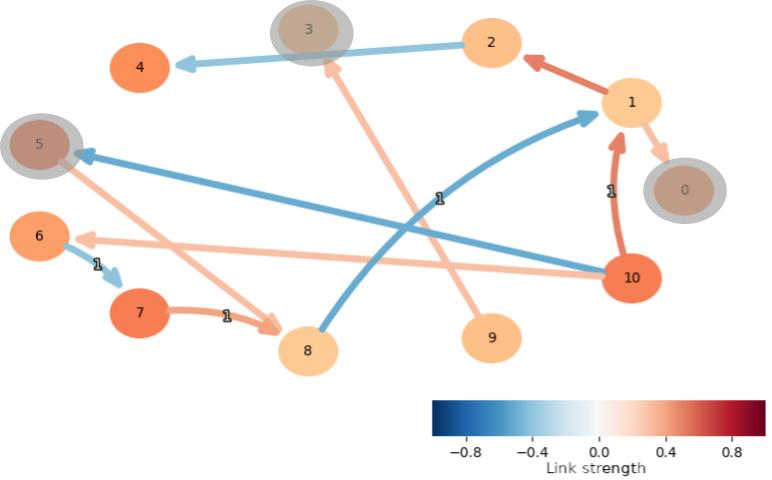
\includegraphics[width=0.32\linewidth]{figs/3_latent.jpg}
    }
             \subfigure[Oracle PAG, which serves as ground truth. It satisfies all conditional independence information of the observed DAG perfectly.]{
   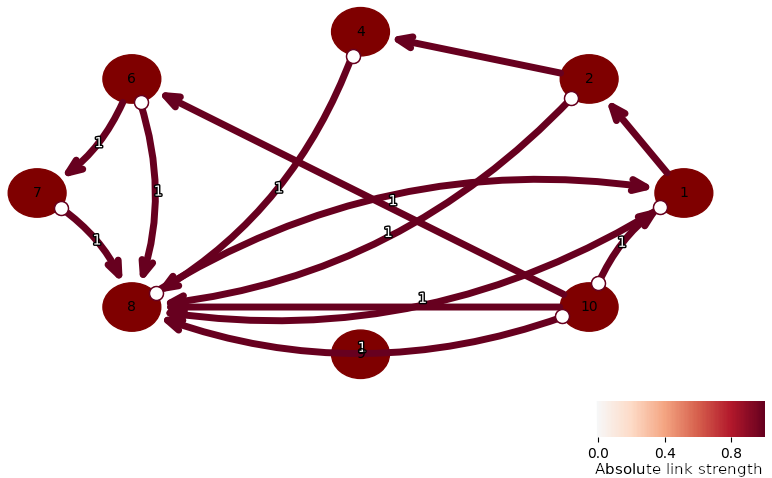
\includegraphics[width=0.32\linewidth]{figs/4.png}
    }
    \subfigure[Predicted PAG that LPCMCI returns.]{
    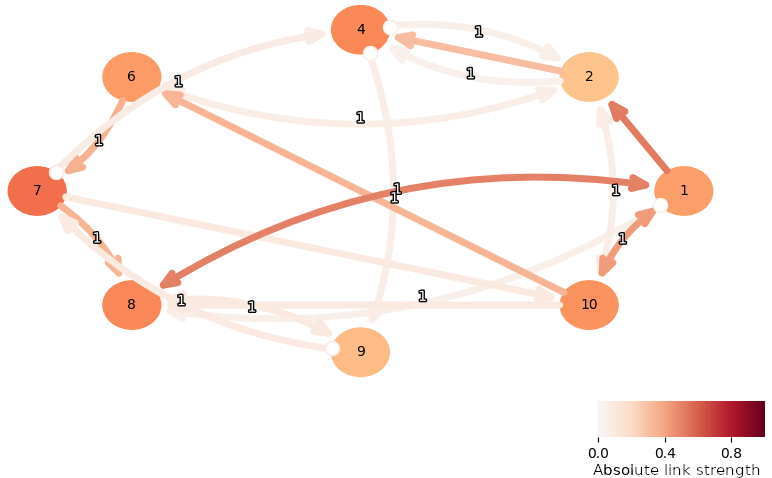
\includegraphics[width=0.32\linewidth]{figs/5_1.png}
    }
    \caption{Oracle and predicted PAG}
        \label{fig:predicted}
\end{figure}

% % removed weak links
% \begin{figure}[htbp]
%     \centering
%     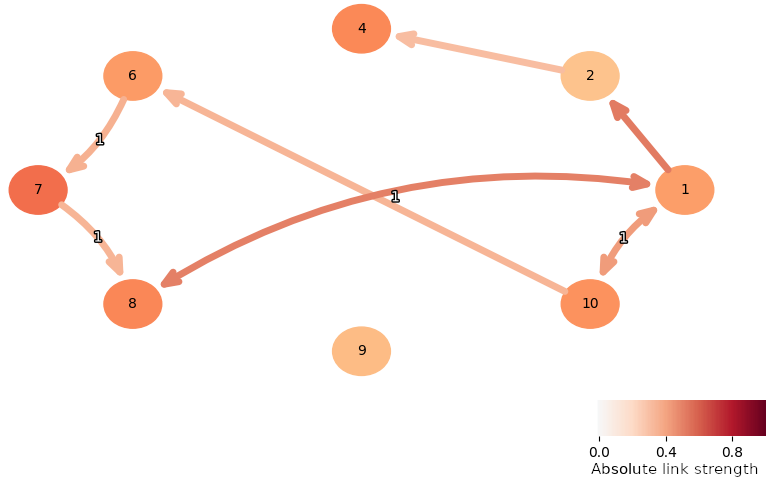
\includegraphics[width=0.6\linewidth]{figs/6.png}
%     \caption{removed weak links
%     \label{fig:removed}
% }
% \end{figure}



\section{Limitations and future work}
\textcolor{red}{stationarity, trends, , changes in variance. seasonality, age, }
%=============================================================================
A measurement frequency slower than the causal processes could violate the assumption of acyclicity of the graph. 
Furthermore, the algorithm is limited to stationarity processes and assumes no selection bias in the data.
In this work, we omitted background knowledge of (non-)ancestorships but planned to use it in future work as we expect that it increases performance.

The evaluation process uses the oracle PAG as ground truth, which in most cases differs from the data-generating DAG. One can see the difference between these two graphs by comparing Figure \ref{fig:predicted}(a) and Figure \ref{fig:predicted}(b). The downside of evaluating against the oracle PAG is that a perfect prediction of the data-generating DAG would usually not receive a perfect score.

Figure \ref{fig:removed} shows that the predicted PAG (b) has many false positives with a weak link strength when evaluating against the data-generating DAG (a). Figure \ref{fig:removed}(c) shows the predicted PAG where weak links with a strength below 0.10 are removed. In this example of Figure \ref{fig:removed} we observe that removing weak links decreases false positives without increasing false negatives. In future work, we want to investigate this phenomenon in more detail. Moreover, instead of removing weak links at the end, we also want to investigate if it would be helpful to iteratively lower the significance level $\alpha$ to remove false positives without inducing false negatives.

The algorithm only returns the absolute values of the predicted link strength, as one can see in Figure \ref{fig:predicted}. The reason is that it computers the link strength via the p-value. We plan to differentiate between positive and negative link strengths in future work by using a distance correlation metric (e.g., Pearson correlation coefficient in the linear case).



% original DAG
\begin{figure}[htbp]
    \centering
        \subfigure[Original DAG of the data-generating process.]{
    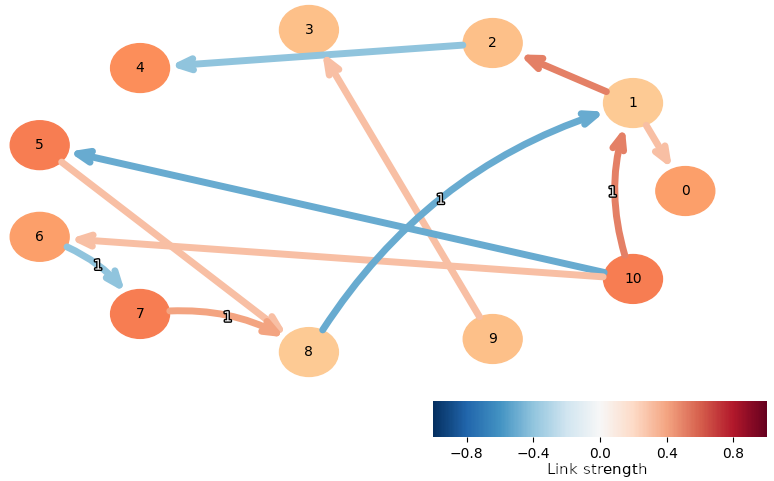
\includegraphics[width=0.3\linewidth]{figs/3.png}
    }
    \subfigure[Predicted PAG]{
    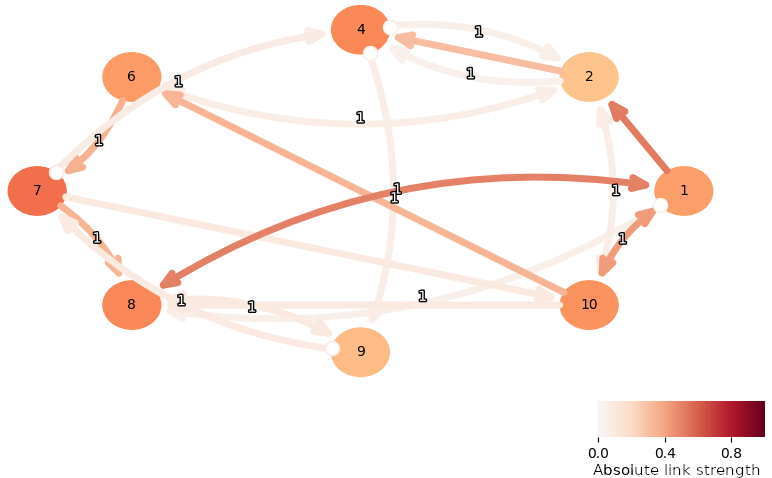
\includegraphics[width=0.3\linewidth]{figs/5_1.png}
    }
    \subfigure[Predicted PAG without weak links.]{
    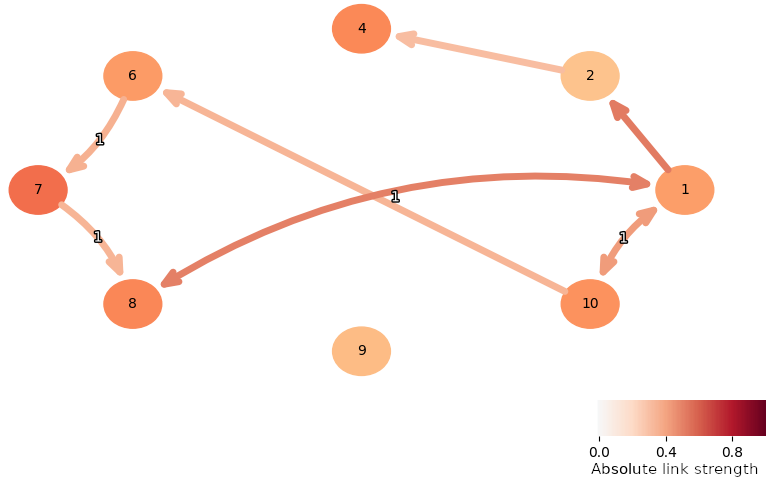
\includegraphics[width=0.3\linewidth]{figs/6.png}
    }
    \caption{Weak links of the predicted PAG tend to be false positives compared to the original data-generating DAG.}
        \label{fig:removed}
\end{figure}


\subsection{Conclusion}
In this work, we generated multi-dimensional time-series with high auto-correlation and latent variables and searched for methods to reconstruct the data-generating process from its observed data.
We briefly explained the advantages and limitations of today's main methods and applied the LPCMCI algorithm.
For our generated datasets, LPCMCI performs best on auto-dependencies, then contemporaneous dependencies, and struggles most with lagged dependencies.

\section{Acknowledgments}
I thank Paul-Christian Buerkner for helpful discussions and suggestions.

%Backmatter
%=============================================================================

\bibliographystyle{IEEEtran}
\bibliography{refs}


%=============================================================================

% \section{Appendix}
% \label{sec:Appendix}



\end{document}
